papers containing reliability in approx. computing


Performances VS Reliability: how to exploitApproximate Computing for Safety-Criticalapplications

Assessing the reliability of successive approximate computing algorithms under fault injection


new TOC 

Introduction:
Approximate computing and reliability:
- approximate computing
    - not novel concept
    - both in software and hardware
    - algorithmic approximations (using math to approach a correct answer; such as integrations (?)
    - dedicated software tools 
        - DSLs 
        - compiler add-ons(TAFFO)
        - runtime tools (?)
        - manual hardcoded approximations
        - approximate algorithms
    - hardware
        - approximate dedicated circuits
        - stochastic computing
        - voltage scaling
        - analog computing circuits
- reliability
    - define through price, 
    - fault tolerance:
        - faults, errors, reliability concept (e.g. fault is reason for error)
    - fault injection
        - software fault injection
            - software fault examples: buffer overflow, referencing pointer that doesn't exist, freeing memory that is still used. 
            - Reason for performing fault injection: e.g. catching coding errors that are not covered by the test cases.    
            - methods of performing fault injection/modes of fault injection:
                - G-SWFIT
                - mutation testing
        - hardware fault injection
            - not focus of paper
            - e.g. bit flipping
            
- Research question:
    - how to measure fault tolerance of software using approximate computing through fault injection

related work: 
- Hardware fault injection in approximate circuits
    - multiple papers 
    - lazers, bit flipping
- software fault injection in approximate computing
    - intrinsic fault tolerance of approximate computing frameworks
    - fault injection in approximate computing not explored deeply
    - mostly focused on operational faults

discussion:
- measuring fault tolerance in approximate computing
    - error = numerical error
    - fault tolerance 
        - which faults? = software faults (relevance = autogenerated code, human generated code)
        - measuring faults: depending on whether faults result in error
        - faults: developmental and operational
        - measurement connected with code test coverage?

conclusion:
- experimental campaign
    - tools that I will base my research on
        - taffo
        - ??
        - goal: cover multiple approaches to approx computing
        - running common benchmarks for common, varied workloads
            - numerical accuracy
            - fault tolerance:
                - how to measure? use existing measures adapted to domain, or generalized measures.
            

In your thesis, we are interested in using "resilience to faults" as performance indicator and numerical accuracy as error estimation.
Can you come up with a list of metrics (i.e., numbers we can count on and plot nice graphs about) that are significant for the resilience aspect?
The last two section of your report should be
- a reflection on these aspects
- a plan for the experimental campaign you will perform during your thesis to extract counters and plot nice graphs

"approximate computing" AND ( "accuracy" OR "precision" ) AND ( tool OR technique OR algorithm ) AND software AND fault AND tolerance

conclusion:
- more work is needed!

% reliability and fault tolerance overview:
%   - definition of faults, fault tolerance and reliability (price et. al.) 
%   - measuring fault tolerance through fault injection
    % - G-SWFIT
%     - quantifying fault tolerance with fault injection
%     - mutation testing

% reliability + approximate computing
%   - related work
%     - 
  
% explaining different types of approximate computing
% - hardware
%   - stochastic/probabilistic computing
%   - voltage (over)scaling
% - software
%   - float -> fixed
%   - approximate algorithms
%   - loop performation
%   - bit width manipulation
%   - ... more?

Examples of approx computing frameworks:

green: loop perforation, function approximation, quality assurance of approx software parts compared with exact parts

approximate computing targeting deep learning networks:





approximate computing : emerging paradigm for energy efficient design
relaxing need for fully precise/deterministic operations, approx computing allows for improved energy efficiency. paper focuses on HARDWARE >:( \cite{han2013approximate} They differentiate between approx. computing: do not assume stochastic nature of underlying processes, deterministic designs that produce imprecise results, often using statistical properties of data and algorithms, and stochastic computing: paradigm that uses random binary bit streams for computation. information is transferred through statistics of the binary stream. Hardware is simple, and fault tolerance is built in. (is this hardware or software fault tolerance? sounds like software). Probabilistic computing: exploiting intrinsic probabilistic behavior of underlying circuit fabric. \cite{han2013approximate}



survey on approximate computing and intrinsic fault tolerance \cite{rodrigues2020survey}
paper on fault tolerance to HARDWARE faults. Fault tolerance is not measured with respect to kinds of software faults created by humans and the errors they produce, only on results of certain computations.




pushing limits: how fault tolerance extends the scope of approximate computing
approximate computing limited to fields with inherent error tolerance. scope of applications has to be significantly extended to other compute intensive domains. the use of fault tolerance measures for these fields are neccessary. paper evaluates techniques that can help extend applicability of approximate computing to fields that typically have higher standards for accuracy. Not using price's definitions of errors and faults.\cite{wunderlich2016pushing}






fault injection measures: 
FARM 
- (set of F(aults) + set of A(ctivations for target system)  => set of R(eadouts collected to characterize the target system behavior in the prescence of faults) ) => M(easures derived from analysis and processing of F,A,R sets) 
readouts for fault tolerance algorithms and mechanisms (FTAM):

\begin{figure}
    \centering
    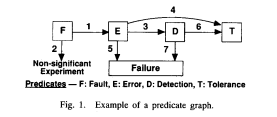
\includegraphics[width=0.5\linewidth]{Images/Readout predicates.png}
    \label{fig:enter-label}
\end{figure}
set of predicates (or combination of predicates) define graph either for anticipated events or after the fact to analyze R set.
other examples of predicates:
{fault-activated}, {faultactivated
errorsignaled} 
statistically evaluating error tolerance to get a number of how error tolerant application is\cite{arlat1993fault}



Classification of faults:  Orthogonal Defect Classification
Assignment: values assigned incorrectly / not assigned
checking: missing validation of parameters or data in conditional statements
Algorithm: efficiency or correctness problems that can affect the taks and be   
    fixed by reimplementing algorithm or local data structure without need for requesting design change
Timing/serialization: needed serialization of resource is missing, wrong resource 
    serialized or wrong form of serialization
Interface: communication problem between services (laprie)
Function: affects larger amount of code, refers to incorrectly implemented  
    capability or incorrectly implemented capability

triggers are the places we want to look for faults that can cause errors.
- startup/restart
- workload volume/stress
- recovery/exception 
- Hardware/software config (relating to unexpected configurations)
- normal mode (no external conditions must apply for fault to turn into error, paper mentions this implies another underlying trigger)
\cite{christmansson1996generation}


G-SWFIT: defining operator library specifying patterns. Code changes must be defined prior to the injection of emulated faults, injection is carried out in executable code. \cite{duraes2006emulation}












definition of faults: \cite{shivakumar2014architecting}
Software fault tolerance
Software faults are due to various reasons. A few critical failure scenarios are given below:

• The application module fails to scale during a heavy load. It could consume high CPU and memory and could exhaust the entire heap memory at higher workloads

• The enterprise integration component fails to establish connection with the upstream and may fail

• The application method was not designed to handle the input data and can cause runtime error.

There could be a variety of software faults due to design-time and runtime issues. Normally, exception handling routines will be developed to catch any expected or unexpected errors. However, the crucial difference between an exception handling routine and a fault-tolerant routine is that exception handlers can stop or continue processing, which does not guarantee the expected functionality as per the specification. But a fault-tolerant procedure should be robust enough to detect and handle the faults in such a way that end functionality is as per the specification. In other words, the end user would not see any difference, with or without faults.

Let us look at the ways to handle the software faults:

• Application code analysis and fault handlers: During application integration testing, use the code profiling tools to carefully analyze the scalability of each component in different layers. By loading each layer, analyze the behavior of the components in those layers and check the consumption of CPU/memory and network resources by those software components. If the consumption of CPU or memory of any of the components increases in exponential scale or on higher proportion to the increased load, it should be redesigned to handle the resources in an optimal way.

While application code analysis would detect potential error scenarios during the testing phase, there must be robust software fault handlers to take care of unhandled software faults at runtime. For instance, if a file parser utility is not efficiently designed to parse a large file, then it could crash when parsing a huge file. Similarly, a data handler utility may not scale up while processing huge a data set from the database. As these are runtime scenarios, they would be difficult to be detected during the testing phase. To handle such scenarios, fault handlers should be designed to detect and prevent the fault before it occurs. A fault handler provides fault-handling capability by performing two tasks:
• It monitors the software components for known fault scenarios. Though software faults could occur due to variety of reasons, we can categorize the underlying cause into fewer high-level categories. Some key fault-causing categories include components and operations that cause memory exhaustion, CPU overutilization, excessive object creation, and poor garbage collection/memory cleanup, high network utilization, and such. These fault causes act as signature markers for early detection of potential faults. Fault handlers will be designed to detect early warning signs of these fault markers. For example, if any software module suddenly starts consuming an excess amount of CPU or memory, the fault handler will immediately notice this abnormality.

• The fault handler will then stop the processing of that faulty module and switch to a different version of the software module to achieve the functionality. The switch will be transparent to the end user with little overhead on request processing. Each critical component that is used in the request processing chain will have different versions, each of which has a distinct design for implementations. This is similar to the N-version software, which is discussed next. A different version of the component hopefully will not create the same fault condition due to its difference in design and implementation.


• Recovery using checkpoint and rollback: This technique is mainly used for data-intensive systems wherein the software always creates a checkpoint of data during its consistent/stable state. The application stores its entire state into a persistent storage at regular intervals. For optimization purposes, subsequent checkpoints can only store the differential data from its previous checkpoint. During a fault scenario, the fault handler routine detects the fault and rolls back the application state to the last-known checkpoint, which contains a valid consistent application state. Though this technique is widely used in database and operating system routines, the same technique can also be used for application software. A data-driven web application can persist its user session data into persistent storage at regular intervals. Each storage will be identified by its timestamp and user details. When a user session is corrupted due to security incidents or other unforeseen circumstances, the fault handler can recreate the user session from the previously known valid checkpoint data. This technique can be utilized for applications having long use sessions and transactions such as report generations, multistep transactions, and long running process workflows.

• N-version software: This technique mimics n-version redundant hardware, and it involves creating n different implementations of the same software module. Each version of software component is designed and implemented in a different way. A more robust version of this design involves having each version of the software component in a different environment, using a different programming language, and each using a completely different design. The probability of failure would reduce due to this design diversity. Another requirement is that each component should strictly conform to the design specifications so that a component switching module can choose among any version of the available components.

• Fault handling through fallback: Though this is not a strict fault-tolerant technique, it is widely used to minimize the impact caused by critical errors on the end user. This technique involves creating fallback mechanisms for every critical process and transaction. Fault handlers invoke fallback procedures to take an alternate course of action. Following are some of the fallback procedure examples:
• If the requested resource is unavailable, load the file from local storage or from the persistent cache. For instance, if the website relies on a crucial taxonomy file, and if the file is unavailable or is corrupted, the fault handler will store and use a local version of the taxonomy file.

• If one of the functionalities is failing, provide a graceful degradation of the functionality. For instance, in an e-commerce application, if the product price cannot be retrieved due to unavailability of the pricing system, display the product without pricing. Similarly, if any of the back-end services are down, get the last-known values from the shared cache.

Designing fault-tolerant routines involves various aspects such as providing alternate processing during heavy loads, smart distribution of requests, fallback procedures to take alternate course of action, and graceful degradation of functionality. In the scalability context, a fault-tolerant system needs to support the main functionality even if some of its components fail. However, there could be partial loss of functionality or increased response time. To summarize, software fault tolerance can be achieved by two main ways:

1.
Adding redundant software components and creating n-version software modules

2.
Designing fallback routines, which sense the component failure and execute an alternate course of action with available components.

Hardware fault tolerance
Fault tolerance at hardware is relatively standardized when compared to software fault tolerance. It depends mainly on these attributes:

• Hardware component redundancy: The infrastructure can be made more robust by adopting N+1 or N+M design wherein, for each distinct hardware component, such as web server node or database node, there will be an additional redundant component with the exact, same configuration. A multi-node cluster is a classic example of this redundancy, wherein the cluster has multiple computing nodes with similar configurations, with one being primary and others being secondary nodes.

Redundancy can be achieved at various levels. Redundancy can be achieved at other levels as well:
• Node level: Redundant components will be used for each distinct computational node. Distinct servers such as the web server, application server, and database server will have multiple instances in a clustered configuration. Similarly, storage devices and content management system (CMS) servers will have redundant nodes.

• Cluster level: We can have the live cluster, which is serving the request, and a standby passive cluster. A standby cluster contains all nodes with configurations similar to the live cluster. A load balancer will use the standby cluster when the live cluster is down.

• Site level: A redundant site, which is similar to the primary site, can be created to handle unforeseen disasters. This is the normal strategy for disaster recovery (DR) and business continuity.


• Replication: In addition to having redundant components, it is important to have the data and configuration in the redundant nodes are exactly the same as their primary counterparts. This is important for effective failover strategy. Replication in its simple form is just synchronization of data and configuration across primary and redundant nodes. There are two main types of replication:
• Synchronous: The data and configuration are replicated simultaneously between primary and all redundant components. This is done to keep all computing nodes in continuous sync. This is normally done for transaction-intensive systems where data freshness and integrity are of prime importance.

• Asynchronous: Data and configuration replication happen in asynchronous fashion. This replication will be more efficient because it reduces the load on the source system, and we can synchronize only the incremental data. Data synchronization can be executed in batch mode during the most suitable time for the application when the traffic is lowest. This technique is normally implemented using scheduled off-line batch jobs.


• Fault detection and isolation: This involves continuous status monitoring of all components, to identify the component that has faulted. Usually, cluster managers or node managers will be responsible for detecting the status of nodes. At a higher level, the load balancers and cluster managers will do this job to check if the cluster or a site is or is not responding. In some instances, even custom health check monitors will be used to identify the faulty nodes. Various techniques are used to test the status of nodes:
• Regular heartbeat messages to check the status of the server. For instance, a web server status can be determined by making an HTTP request and looking for an HTTP response code

• Regular ping messages

• Custom health check URLs, function, and service calls
• Continuous analysis of response times of servers. A gradual degradation of response trend hints at a fault in a short period of time

Isolation of a fault is a tricky business in the case of n-tier application. We need to use custom health check monitors that check the servers at each layer and then drill down to the root cause. For example in a regular three-tier application, check the status and health of the web server and then move to the application server, then to the database server, and so on.

• Failover: Once a fault is identified with a particular component, the requests must be transparently failed over to the healthy nodes. Load balancers and cluster managers use a variety of techniques to fail over to other nodes:
• The faulty node that is not responding is marked as offline, and the node status is updated accordingly. No requests will be served to them until it is in offline mode.
• All future requests will be served to secondary redundant nodes, which are in standby mode.
For the failover to be successful, data should be replicated to the redundant nodes on a regular basis; this is a prerequisite for the failover. Also, requests that have less session stickiness will be easy to switch.









